\chapter{Implementación}

En este capítulo se mostraran los fundamentos mas importantes sobre la implementación tanto del front-end como del back-end y de como montar un instalador para Windows.

\subsection{Implmentación del front-end}

En esta sección se explicaran cuales son las configuraciones más importantes de Angular.js porque este es el más importante del front-end. 

\subsubsection{Organización y carpetas}

La capeta public es la que contiene todo lo relacionado con el front-end del simulador de escenarios. Dento de este encontramos la siguiente estructura de directorios: 

\dirtree{%
	.1 Simulator.
	.2 public.
	.3 images.
	.3 javascript.
	.4 angular.
	.4 bootstrap.
	.4 jquery.
	.4 openlayers.
	.4 socketsIO.
	.3 stylesheets.
	.3 views.
}

A continuación vamos a ver cual es la función de cada uno de estos directorios:
\begin{itemize}
	\item images: contiene imágenes estáticas que se están utilizando en la aplicación.
	\item javascript: contiene todos los frameworks de javascript que se están utilizando en el front-end. Hay una carpeta para cada framework.
	\item javascript/angular: contiene todas las configuraciones de Angular.js. Este tiene 4 subdirectorios: config (contiene el router de Angular.js), controllers (contiene los controladores de Angular.sj), factory (contiene el factory de Angular.js) y services (contiene los servicios de Angular.js).
	\item javascript/bootstrap: contiene el sistema de componentes de bootstrap.
	\item javascript/openlayers: contiene el framework de OpenStreetMap.
\end{itemize}

\subsubsection{El router de Angular.js}

El router de Angular.js es el encargado del direccionamiento dentro de la página. En las configuraciones de este vinculamos una URL con una vista y esta con un controlador. Podemos encontrar las configuraciones de este en la carpeta /public/javascript/angular/config/routes.js:

\begin{lstlisting}[language=xml, frame=single]
var app = angular.module("app", ['ngRoute', 'ngStorage', 'checklist-model', 'xeditable']);

app.config(['$routeProvider', '$httpProvider' ,function($routeProvider, $httpProvider) {	 		   
$routeProvider.when('/', {
templateUrl: 'views/index.html',
controller: 'LoginController'
}).when('/register', {
templateUrl: 'views/register.html',
controller: 'RegisterController'
}).when('/map', {
templateUrl: 'views/maps/index.html',
controller: 'MapController'
}).when('/map/newMap', {
templateUrl: 'views/maps/newMap.html',
controller: 'NewMapController'        
}).when('/map/editScene', {
templateUrl: 'views/maps/editScene.html',
controller: 'EditSceneController'        
}).when('/map/editMap', {
templateUrl: 'views/maps/editMap.html',
controller: 'EditMapController'
}).when('/simulator', {
templateUrl: 'views/simulator/index.html',
controller: 'SimulatorController'
}).when('/settings', {
templateUrl: 'views//settings/recommenderSettings.html',
controller: 'RecommenderSettingsController'
}).when('/settings/staticItemSettings', {
templateUrl: 'views/settings/staticItemSettings.html',
controller: 'StaticItemSettingsController'
}).when('/settings/dynamicItemSettings', {
templateUrl: 'views/settings/dynamicItemSettings.html',
controller: 'DymanicItemSettingsController'
}).when('/profile', {
templateUrl: 'views/configurations/index.html',
controller: 'ConfigurationController'
}).otherwise({
redirectTo: '/'
}); 

$httpProvider.interceptors.push(['$q', '$location', '$localStorage', function($q, $location, $localStorage) {
return {  
'request': function (config) {    
config.headers = config.headers || {};

if ($localStorage.token) {
config.headers.Authorization = 'Bearer ' + $localStorage.token;
}

return config;

},

'responseError': function(response) {
if(response.status === 401 || response.status === 403) {
$location.path('/signin');
}

return $q.reject(response);
}
};    
}]);    
}]);
\end{lstlisting}

En el mismo fichero tenemos configurado también un interceptor. El interceptor es un método que se ejecuta cada vez que llega o sale una petición. En nuestro caso el interceptor es utilizado para encriptar y desencriptar los datos involucrados en la comunicación. También es el encargado de poner la cabecera Authorization que se utiliza para autentificar el usuario en cada petición.

\subsubsection{Los controladores de Angular.js}

Los controladores de Angular.js contienen la lógica de las vistas y establecen la comunicación con el back-end mediante los servicios de Angular.js. Existe un controlador por cada página y contiene funciones y datos propias de la vista. Como regla general se ha establecido que el nombre de controlador es el mismo que la vista a la que va asociada pero acabado con la palabra clave Controller. Podemos encontrar todos los controladores en la carpeta /public/javascript/angular/controllers.  

\begin{figure}[H]
	\centering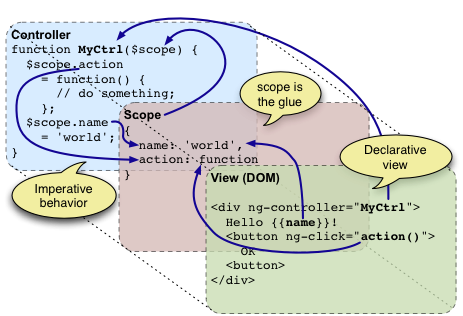
\includegraphics[scale=0.5]{imagenes/concepts-controller.png}
	\caption{Ejmplo de un controlador}
	\label{controllerExample}
\end{figure}

Según la filosofía de Angular.js las vista se actualizan de forma automática cuando actualizamos el modelo de datos del controlador. A continuación podemos ver un diagrama a cerca de como funciona:

\begin{figure}[H]
	\centering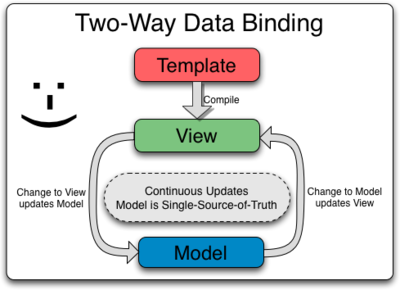
\includegraphics[scale=0.5]{imagenes/twoway.png}
	\caption{Two-way data binding}
	\label{twoWayDataBinding}
\end{figure}

\subsubsection{Los servicios de Angular.js}

Tener toda la lógica metida en los controladores y en el modelo de datos no es buena idea porque cuando la aplicación empieza a crecer se complican las cosas.

Los servicios son un concepto importante en Angular.js porque nos permiten agrupar funcionalidades que luego estarán disponible en los controladores, mejorando la claridad del código y favoreciendo la reutilización.

En nuestro caso hemos agrupado las llamadas al back-end y accedemos a la información del usuario autentificado desencriptada por los interceptores. Podemos encontrar todas las configuraciones de los servicios en el fichero /public/javascripts/angular/services/Services.js.

\subsection{Implmentación del back-end}



\subsection{¿Como montar un instalador de la aplicación?}


